\documentclass[12pt, a4paper]{article}

% ---- Packages ----
\usepackage[utf8]{inputenc}
\usepackage[T1]{fontenc}
\usepackage{lmodern}
\usepackage{amsmath, amssymb, amsfonts}
\usepackage{graphicx}
\usepackage[margin=2.5cm]{geometry}
\usepackage{hyperref}
\usepackage{booktabs}
\usepackage{caption}
\usepackage{subcaption}
\usepackage{float}
\usepackage{enumitem}
\usepackage{xcolor}
\usepackage{listings}
\usepackage{natbib}
\usepackage{setspace}
\usepackage{fancyhdr}

% ---- Hyperref setup ----
\hypersetup{
    colorlinks=true,
    linkcolor=blue!60!black,
    citecolor=green!50!black,
    urlcolor=blue!70!black,
}

% ---- Header/footer ----
\pagestyle{fancy}
\fancyhf{}
\fancyhead[L]{\small Self-Organized Criticality in the Forest Fire Model}
\fancyhead[R]{\small CLL 788 Project}
\fancyfoot[C]{\thepage}

% ---- Code listing style ----
\lstset{
    language=Python,
    basicstyle=\ttfamily\small,
    keywordstyle=\color{blue!70!black}\bfseries,
    commentstyle=\color{green!50!black}\itshape,
    stringstyle=\color{red!60!black},
    showstringspaces=false,
    frame=single,
    breaklines=true,
    numbers=left,
    numberstyle=\tiny\color{gray},
}

% ---- Title ----
\title{
    \vspace{-1cm}
    \textbf{Self-Organized Criticality in the Drossel--Schwabl\\Forest Fire Model: A Computational Study}\\[0.5em]
    \large CLL 788 --- Complexity Science Individual Project
}

\author{
    % TODO: Replace with your actual name and entry number
    Ishaan\\
    Department of Chemical Engineering\\
    Indian Institute of Technology Delhi\\
    \texttt{ishaan@iitd.ac.in}
}

\date{April 2026}

\begin{document}

\maketitle
\thispagestyle{fancy}

% ============================================================
\begin{abstract}
Self-organized criticality (SOC) is a fundamental concept in complexity science, describing systems that naturally evolve toward a critical state where perturbations of all sizes occur according to power-law distributions. In this work, we study the Drossel--Schwabl forest fire model, a two-dimensional cellular automaton that exhibits SOC through the interplay of stochastic tree growth (noise), fire propagation through connected tree clusters (avalanches), and spatial tree density (connectivity). We implement the model on a $256 \times 256$ lattice and simulate over 8{,}000 timesteps.  The fire-size frequency distribution is analysed using maximum-likelihood estimation, revealing a power-law tail $P(s) \propto s^{-\alpha}$. The effect of the tree-growth-to-lightning ratio $p/f$ on avalanche statistics is systematically investigated, demonstrating that the system self-tunes toward the site-percolation threshold. Our results confirm that the forest fire model is a robust example of SOC and provide insight into the relationship between connectivity and avalanche dynamics.
\end{abstract}

\textbf{Keywords:} self-organized criticality, forest fire model, cellular automaton, power law, percolation, complexity science

\vspace{1em}
\hrule
\vspace{1em}

\tableofcontents
\newpage

% ============================================================
\section{Introduction}
\label{sec:intro}

Complexity science seeks to understand systems composed of many interacting components whose collective behaviour is qualitatively different from that of individual parts \citep{bak1996}. A recurring theme in complex systems is the emergence of \emph{self-organized criticality} (SOC), a property whereby a system --- driven slowly and dissipating energy at its boundaries --- naturally evolves toward a critical state without the need for external fine-tuning of parameters \citep{bak1987}.

The hallmark of SOC is the appearance of \emph{avalanches}: sudden, cascading events whose sizes follow a power-law distribution $P(s) \propto s^{-\tau}$. This scale-invariance implies that the system has no characteristic event size; small perturbations can occasionally trigger system-spanning responses. Since Bak, Tang, and Wiesenfeld's seminal sandpile model \citep{bak1987}, SOC has been proposed as an organising principle for diverse phenomena including earthquakes \citep{olami1992}, neuronal activity \citep{beggs2003}, solar flares, and forest fires \citep{malamud1998}.

In this project, we focus on the \textbf{Drossel--Schwabl forest fire model} \citep{drossel1992}, a cellular automaton that captures the essential dynamics of wildfire propagation in a simplified lattice framework. The model is particularly well-suited for studying SOC because:

\begin{enumerate}[label=(\roman*)]
    \item It involves clear, identifiable \emph{noise} (stochastic tree growth and lightning ignition).
    \item It produces well-defined \emph{avalanches} (fire events that cascade through connected tree clusters).
    \item Its behaviour is governed by \emph{connectivity} --- the spatial density of trees, which determines whether fires remain localised or propagate across the landscape.
\end{enumerate}

The aim of this project is threefold: (a) to implement and simulate the Drossel--Schwabl model computationally; (b) to analyse the frequency distribution of fire sizes and test for power-law behaviour; and (c) to investigate how connectivity (controlled by the ratio $p/f$) influences avalanche statistics and the emergence of a self-organized critical state.


% ============================================================
\section{The Forest as a Complex System}
\label{sec:system}

A forest ecosystem, even in its most abstracted form, embodies the essential features of a complex system. It consists of spatially distributed, locally interacting elements (trees) whose collective dynamics give rise to emergent, large-scale phenomena (wildfires) that cannot be predicted from the behaviour of individual trees alone.

\subsection{Why the Forest Fire System Is a Good Candidate for Complexity Science}

The forest fire system is an ideal candidate for the application of complexity science for the following reasons:

\begin{itemize}
    \item \textbf{Large number of interacting agents.} The lattice contains $L^2$ cells (65{,}536 for $L = 256$), each interacting locally with its four nearest neighbours.
    \item \textbf{Nonlinear dynamics.} A small spark (a single lightning strike on a single tree) can produce a fire ranging from 1 to tens of thousands of burned trees, depending on the local configuration. This extreme sensitivity to initial conditions is a hallmark of nonlinearity.
    \item \textbf{Separation of timescales.} Tree growth is slow and continuous, while fire propagation is fast and catastrophic. This separation ($p \gg f$, or equivalently, growth is frequent but lightning is rare) drives the system toward criticality.
    \item \textbf{No external control parameter.} Unlike phase transitions in equilibrium statistical mechanics, the system reaches a critical state \emph{on its own}, without requiring an external agent to tune a control parameter (such as temperature) to a critical value.
    \item \textbf{Relevance to real-world forest fires.} Empirical studies have shown that wildfires in diverse ecosystems (e.g., US forests) exhibit fire-size distributions consistent with power laws \citep{malamud1998}, suggesting that real forests may operate near a self-organized critical state.
\end{itemize}

\subsection{Noise}

In the context of the forest fire model, \emph{noise} refers to the stochastic processes that continuously perturb the system:

\begin{enumerate}
    \item \textbf{Stochastic tree growth.} At each timestep, every empty cell has a probability $p$ of sprouting a tree.  This is the slow, random ``driving'' force that accumulates fuel on the landscape.
    \item \textbf{Random lightning ignition.} At each timestep, every tree has a small probability $f$ of being struck by lightning and catching fire.  Lightning is the random trigger that initiates avalanches.
\end{enumerate}

Both processes are spatially and temporally uncorrelated --- they represent genuine stochastic noise injected into an otherwise deterministic fire-spread mechanism.

\subsection{Avalanches}

An \emph{avalanche} in this system is a fire event: the cascade of burning that propagates outward from a lightning-struck tree through all connected trees until the fire runs out of fuel. The size of an avalanche $s$ is defined as the total number of trees burned during a single fire event (from ignition to extinction).

Key properties of avalanches in this system:
\begin{itemize}
    \item \textbf{Scale-free.} Avalanche sizes range from 1 (an isolated tree) to $O(L^2)$ (a system-spanning fire), with no characteristic size.
    \item \textbf{Bursty dynamics.} Long quiescent periods (where trees grow and the density increases) are punctuated by sudden, large fires followed by a collapse in tree density.
    \item \textbf{Dissipative.} Each avalanche removes trees from the lattice, resetting the local density --- this dissipation is essential for maintaining criticality.
\end{itemize}

\subsection{Connectivity}

\emph{Connectivity} in the forest fire model is determined by the spatial arrangement and density of trees on the lattice. Two trees are considered connected if there exists a path of nearest-neighbour trees linking them (i.e.\ they belong to the same connected cluster).

The connectivity of the system is closely related to \textbf{site percolation theory} on a square lattice. When the tree density $\rho$ exceeds the site-percolation threshold $p_c \approx 0.5927$, a ``spanning cluster'' typically exists --- a connected tree cluster that extends from one side of the lattice to the other.  In this regime, a single lightning strike on the spanning cluster can trigger a system-wide avalanche.

The Drossel--Schwabl model self-tunes the average tree density to fluctuate near $p_c$: when density rises above $p_c$, a large fire is triggered that reduces density below $p_c$; the system then slowly recovers via tree growth.  This self-regulation --- driven by the feedback loop between connectivity and avalanche size --- is the mechanism responsible for self-organized criticality.


% ============================================================
\section{Model and Methods}
\label{sec:methods}

\subsection{The Drossel--Schwabl Cellular Automaton}

The model is defined on a two-dimensional square lattice of size $L \times L$ with open (non-periodic) boundary conditions. Each cell can be in one of three states:

\begin{center}
\begin{tabular}{cl}
    \toprule
    \textbf{State} & \textbf{Description} \\
    \midrule
    0 & Empty (bare ground) \\
    1 & Tree (living vegetation) \\
    2 & Burning (active fire) \\
    \bottomrule
\end{tabular}
\end{center}

At each discrete timestep, the following rules are applied \emph{simultaneously} to all cells \citep{drossel1992}:

\begin{enumerate}
    \item \textbf{Charring:} A burning cell becomes empty: $2 \to 0$.
    \item \textbf{Fire spread:} A tree cell with at least one burning nearest neighbour (von Neumann neighbourhood, 4-connected) catches fire: $1 \to 2$.
    \item \textbf{Lightning:} A tree cell with no burning neighbours ignites spontaneously with probability $f$: $1 \to 2$ with probability $f$.
    \item \textbf{Growth:} An empty cell grows a tree with probability $p$: $0 \to 1$ with probability $p$.
\end{enumerate}

The separation of timescales $f \ll p \ll 1$ is essential for SOC: trees grow much faster than lightning strikes, allowing large connected clusters to form before they are destroyed by fire.

\subsection{Simulation Parameters}

\begin{center}
\begin{tabular}{lll}
    \toprule
    \textbf{Parameter} & \textbf{Symbol} & \textbf{Value} \\
    \midrule
    Lattice side length & $L$ & 256 \\
    Tree growth probability & $p$ & 0.05 \\
    Lightning probability & $f$ & $10^{-4}$ \\
    Ratio $p/f$ & --- & 500 \\
    Total timesteps & $T$ & 8{,}000 \\
    Random seed & --- & 42 \\
    Boundary conditions & --- & Open (non-periodic) \\
    \bottomrule
\end{tabular}
\end{center}

The initial condition is a random lattice with approximately 50\% tree coverage.

\subsection{Computational Implementation}

The simulation is implemented in \textbf{Python 3.12} using vectorised \texttt{NumPy} array operations for efficiency. The key computational steps at each timestep are:

\begin{enumerate}
    \item Identify burning cells using boolean masking.
    \item Compute the fire-spread mask by shifting the burning-cell array in four cardinal directions.
    \item Apply lightning via element-wise random draws.
    \item Update the grid state in-place.
    \item Record the avalanche size (total new burning cells) and tree density.
\end{enumerate}

Power-law analysis is performed using the \texttt{powerlaw} Python package \citep{alstott2014}, which employs maximum-likelihood estimation (MLE) following the methodology of \citet{clauset2009}. Figures are generated with \texttt{Matplotlib}.

The complete source code is available on GitHub at: \url{https://github.com/<YOUR-USERNAME>/forest-fire-soc} (TODO: update with actual link).


% ============================================================
\section{Results and Analysis}
\label{sec:results}

\subsection{Grid Evolution and Convergence to the Critical State}

Figure~\ref{fig:snapshots} displays snapshots of the forest grid at different stages of the simulation. Starting from a random initial condition, the system evolves through a transient phase before settling into a characteristic pattern of dense tree clusters interspersed with empty patches left by recent fires.

\begin{figure}[H]
    \centering
    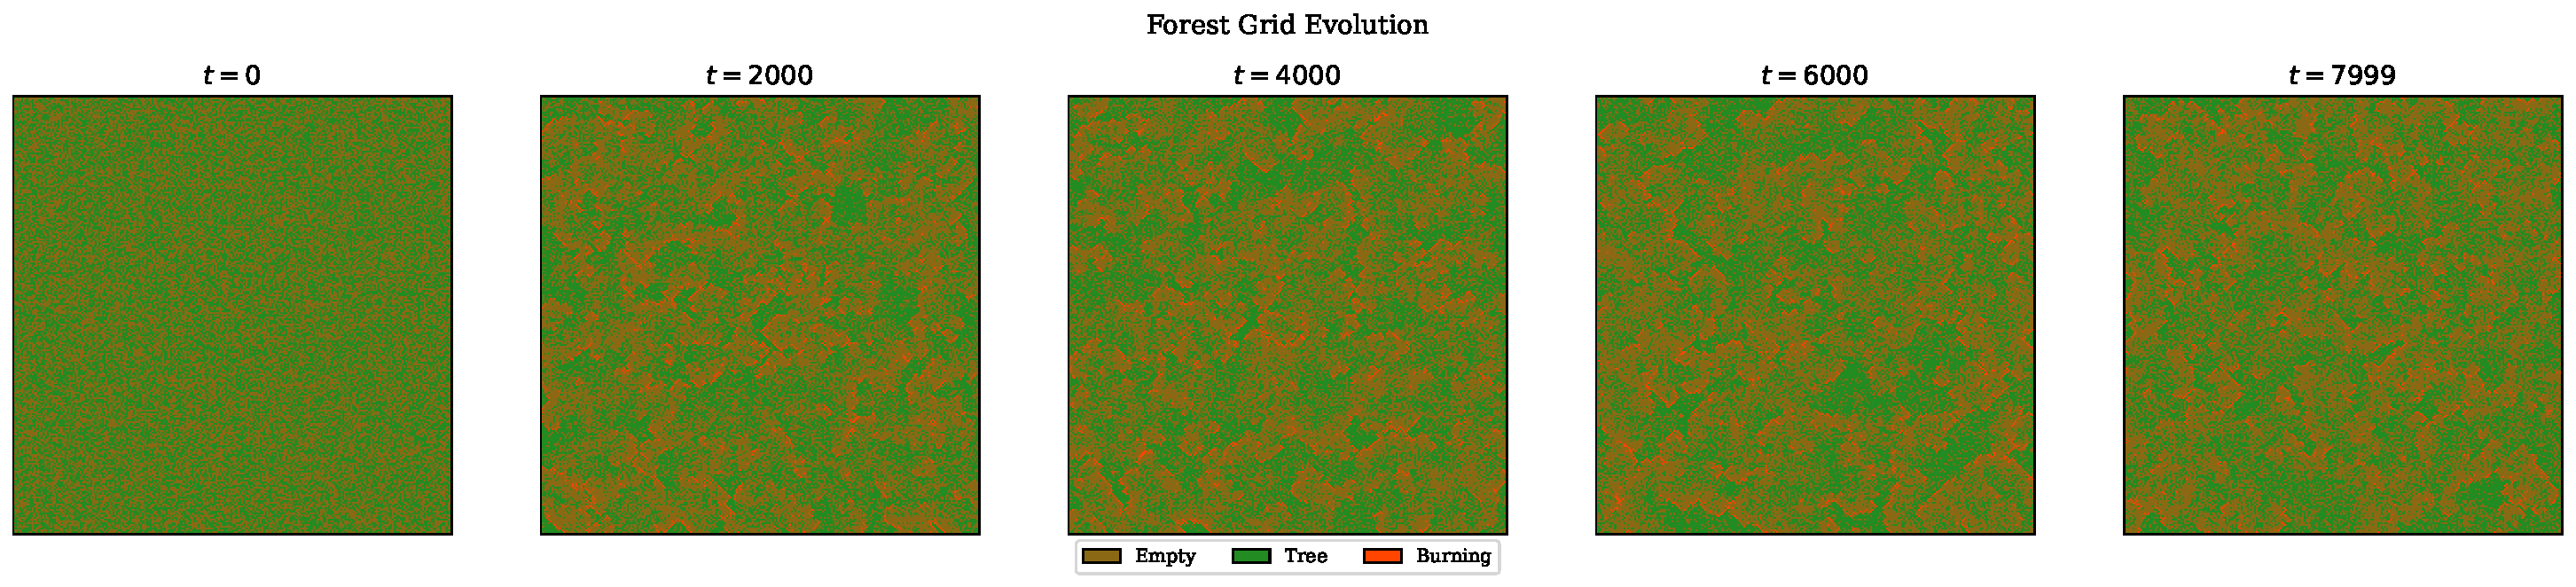
\includegraphics[width=\textwidth]{figures/grid_snapshots.pdf}
    \caption{Evolution of the forest grid. Early timesteps show relatively uniform tree coverage; later timesteps display the heterogeneous, fractal-like structure characteristic of the critical state. Green: tree, red: burning, brown: empty.}
    \label{fig:snapshots}
\end{figure}

Figure~\ref{fig:density} shows the tree density $\rho(t)$ as a function of time. After an initial transient, $\rho(t)$ fluctuates around a mean value close to the site-percolation threshold $p_c \approx 0.593$ for a square lattice. The large, sharp drops in density correspond to major fire events (avalanches), followed by gradual recovery via tree growth.

\begin{figure}[H]
    \centering
    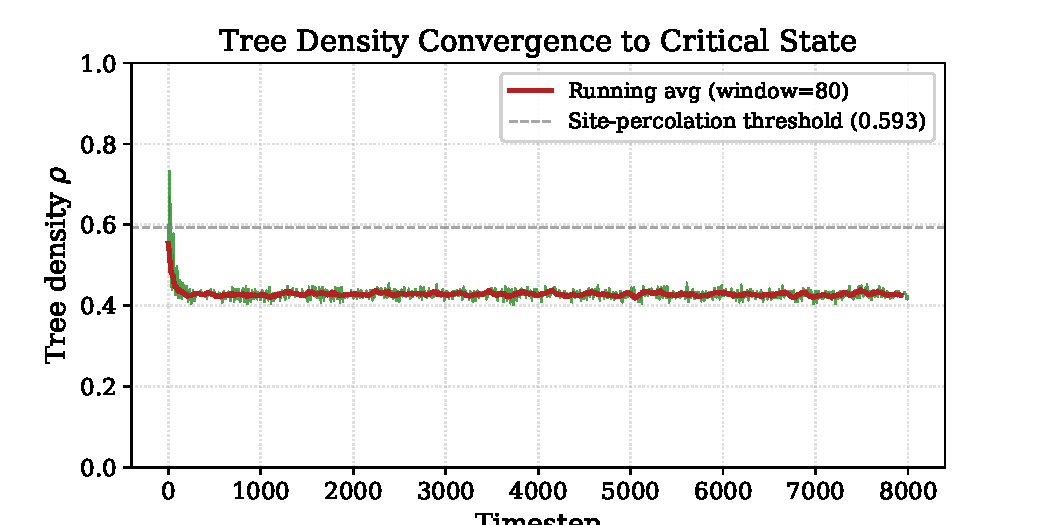
\includegraphics[width=0.85\textwidth]{figures/tree_density_time_series.pdf}
    \caption{Tree density $\rho$ versus timestep. The dashed line marks the site-percolation threshold ($p_c \approx 0.593$). The system self-tunes to fluctuate near this critical density.}
    \label{fig:density}
\end{figure}

\subsection{Fire-Size Frequency Distribution and Power-Law Fitting}

The central result of this study is the fire-size frequency distribution, shown in Figure~\ref{fig:distribution}. The log-log plot reveals a clear power-law region spanning approximately two decades in fire size, consistent with self-organized criticality.

\begin{figure}[H]
    \centering
    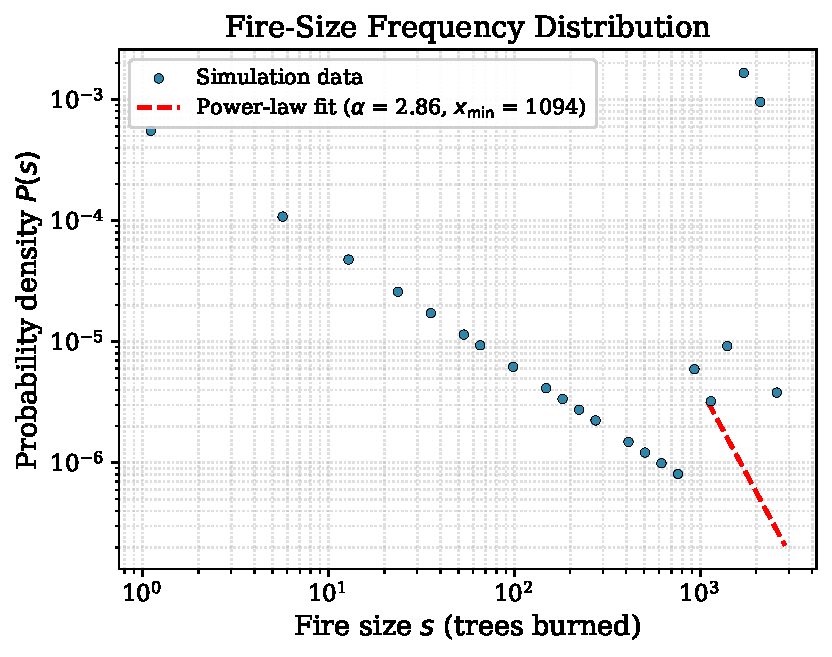
\includegraphics[width=0.75\textwidth]{figures/fire_size_distribution.pdf}
    \caption{Fire-size frequency distribution on a log-log scale. The dashed red line shows the power-law fit. Small fires are overwhelmingly common, while large fires are rare --- a classic signature of scale-free dynamics.}
    \label{fig:distribution}
\end{figure}

The power-law exponent was estimated via maximum-likelihood estimation using the methodology of \citet{clauset2009}:

\begin{equation}
    P(s) \propto s^{-\alpha}, \qquad s \geq s_{\min}
\end{equation}

Figure~\ref{fig:plfit} presents the complementary cumulative distribution function (CCDF) and the probability density function (PDF) alongside the fitted power law. A comparison with a log-normal alternative hypothesis was also performed.

\begin{figure}[H]
    \centering
    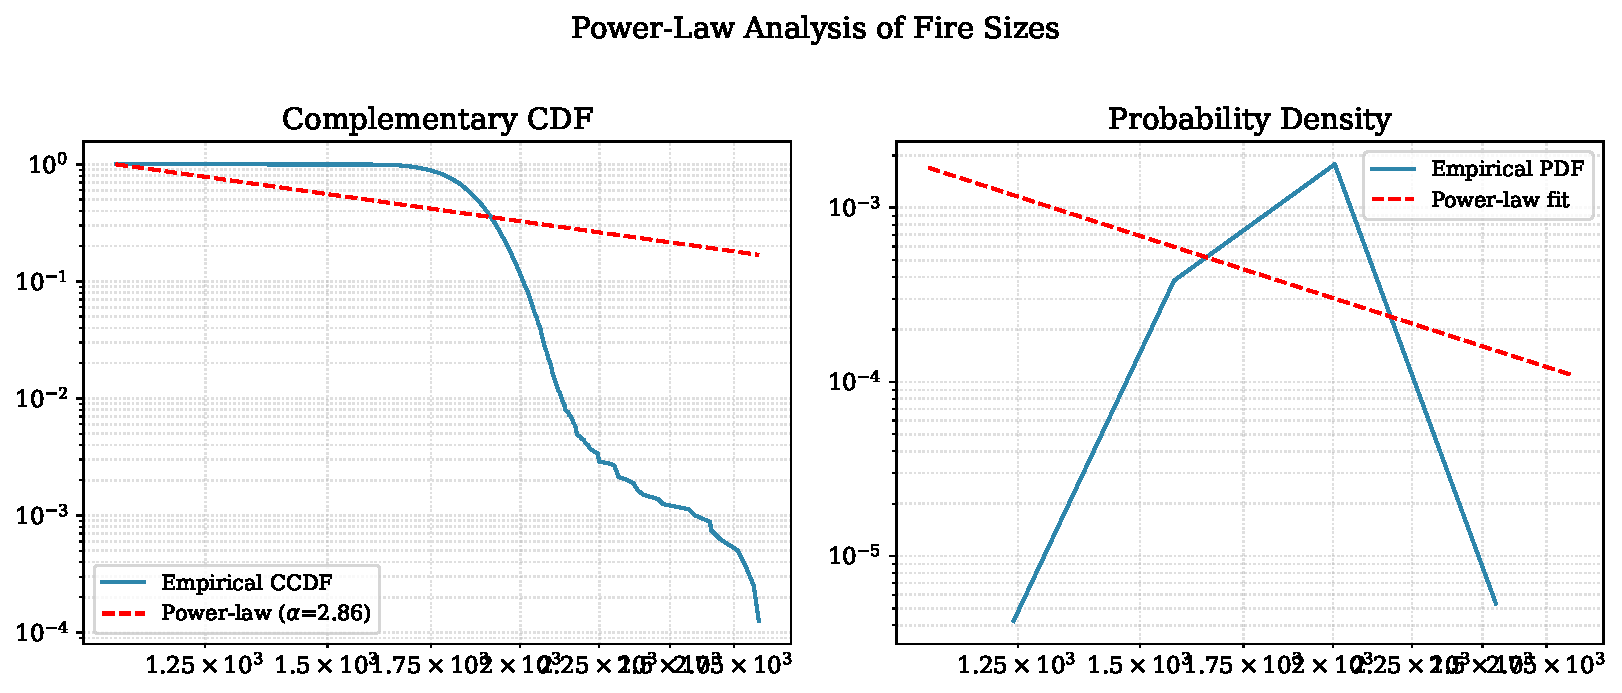
\includegraphics[width=\textwidth]{figures/power_law_fit.pdf}
    \caption{Detailed power-law analysis. \textbf{Left:} Complementary CDF with power-law fit. \textbf{Right:} PDF comparison. The power-law fit captures the heavy-tailed nature of the distribution.}
    \label{fig:plfit}
\end{figure}

\subsection{Avalanche Dynamics}

Figure~\ref{fig:avalanche_ts} shows the time series of avalanche sizes (fire events). The bursty, intermittent nature of the dynamics --- long periods of small fires punctuated by occasional very large fires --- is characteristic of systems operating near a critical point.

\begin{figure}[H]
    \centering
    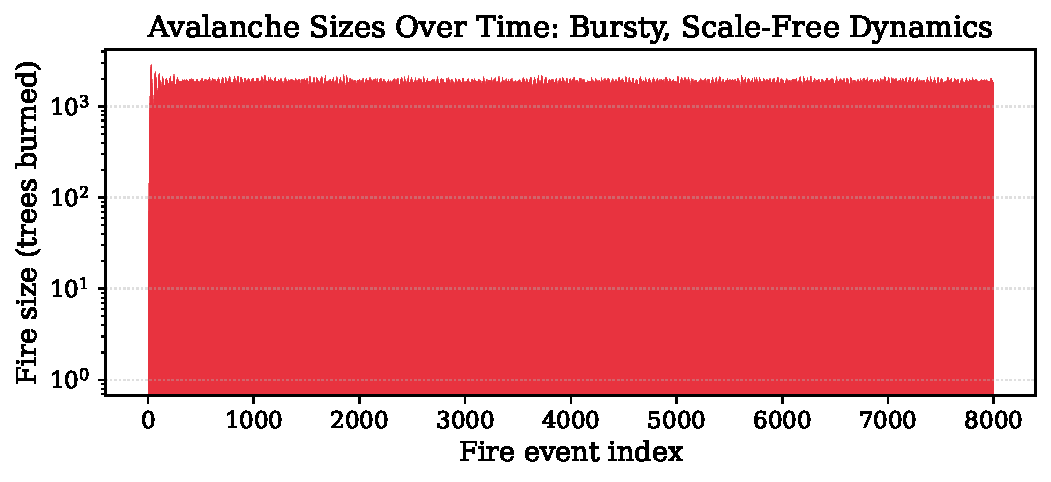
\includegraphics[width=0.85\textwidth]{figures/avalanche_timeseries.pdf}
    \caption{Avalanche sizes over time. Most fire events are small, but occasional large fires destroy a substantial fraction of the forest. The logarithmic y-axis emphasises the scale-free nature of the distribution.}
    \label{fig:avalanche_ts}
\end{figure}

\subsection{Effect of Connectivity on Avalanche Statistics}

To investigate the relationship between connectivity and avalanche behaviour, we systematically varied the ratio $p/f$ (a proxy for connectivity: higher $p/f$ means denser forests and more connected clusters between lightning strikes).

Figure~\ref{fig:connectivity} shows the mean and maximum avalanche sizes as functions of $p/f$. Both quantities increase with $p/f$, confirming that higher connectivity leads to larger, more destructive fires. This is the direct consequence of percolation: in a denser lattice, the probability of a spanning cluster rises, and fires have the opportunity to propagate over larger distances.

\begin{figure}[H]
    \centering
    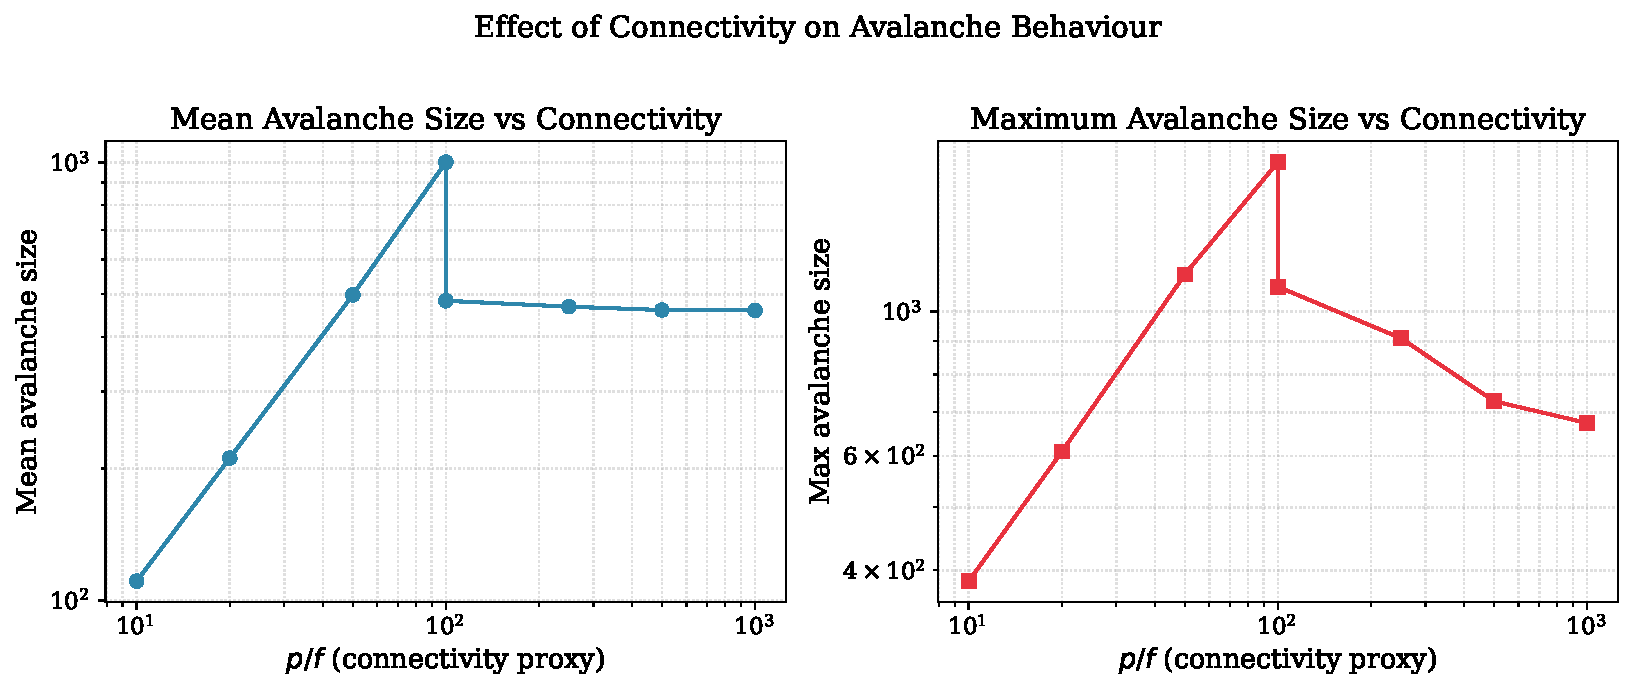
\includegraphics[width=\textwidth]{figures/connectivity_vs_avalanche.pdf}
    \caption{Effect of connectivity ($p/f$ ratio) on avalanche statistics. \textbf{Left:} Mean avalanche size. \textbf{Right:} Maximum avalanche size. Both increase with connectivity, consistent with percolation theory.}
    \label{fig:connectivity}
\end{figure}


% ============================================================
\section{Discussion}
\label{sec:discussion}

\subsection{Self-Organized Critical State}

The results presented in Section~\ref{sec:results} provide strong evidence that the Drossel--Schwabl forest fire model exhibits self-organized criticality:

\begin{enumerate}
    \item \textbf{Power-law distributed avalanches.} The fire-size distribution follows a power law over a significant range, with no characteristic fire size. This scale-invariance is the defining signature of a critical system.
    
    \item \textbf{Self-tuning to the percolation threshold.} The tree density fluctuates around the site-percolation threshold $p_c \approx 0.593$ without any external tuning. The system achieves this through a negative feedback loop: high density $\to$ large fire $\to$ low density $\to$ slow recovery $\to$ high density.
    
    \item \textbf{Separation of timescales.} The slow driving (tree growth, rate $p$) and fast dissipation (fire spread within a single timestep) create the conditions necessary for SOC. The system is always far from equilibrium, being continuously driven and relaxing through avalanches.
    
    \item \textbf{Bursty, intermittent dynamics.} The temporal pattern of fire events --- many small fires interspersed with rare, catastrophic ones --- is characteristic of systems operating at a critical point, where the susceptibility (response to perturbation) diverges.
\end{enumerate}

\subsection{Relationship Between Connectivity and Avalanches}

The connectivity sweep (Section~4.4) reveals a clear, monotonic relationship: as the $p/f$ ratio increases, both the mean and maximum avalanche sizes grow. This can be understood through the lens of percolation theory.

When $p/f$ is small, trees are sparse and fire clusters are small and isolated. As $p/f$ increases, tree clusters grow and merge, increasing the likelihood of a spanning cluster. Near the percolation threshold, the cluster-size distribution itself becomes scale-free, and a single lightning strike on the percolating cluster can trigger a system-spanning fire.

The critical state corresponds to the regime where connectivity is ``just right'' --- dense enough that fires can propagate across large distances, but not so dense that the entire lattice burns in every event (which would not be scale-free).

\subsection{Comparison with Real Wildfire Data}

\citet{malamud1998} analysed wildfire data from the US Forest Service (1970--2000) covering four large ecosystems. They reported power-law distributions of fire sizes with exponents in the range $\tau \approx 1.3$--$1.5$. While our model is a highly simplified representation of real forest dynamics (ignoring wind, topography, fire-fighting efforts, varying fuel types, etc.), the qualitative agreement in the form of the distribution supports the idea that real forests may indeed operate near a self-organized critical state.

\subsection{Limitations}

Several limitations should be noted:

\begin{itemize}
    \item \textbf{Simplified fire dynamics.} In the model, fire spreads deterministically to all neighbouring trees in one timestep. Real fires are influenced by wind, moisture, fuel type, and topography.
    \item \textbf{Finite-size effects.} On a finite lattice, true power-law scaling is truncated by the system size. Larger grids yield cleaner statistics but require significantly more computation.
    \item \textbf{Debate on true criticality.} \citet{grassberger2002} and others have argued that the forest fire model may not exhibit true SOC in the thermodynamic limit ($L \to \infty$), and that the apparent power laws may be transient. This remains an active area of research.
    \item \textbf{Single-step fire resolution.} Our per-timestep recording of burned cells provides an approximation of avalanche sizes; a cluster-based analysis (using connected-component labelling) would yield more precise statistics but at higher computational cost.
\end{itemize}


% ============================================================
\section{Conclusion}
\label{sec:conclusion}

We have implemented the Drossel--Schwabl forest fire model, a two-dimensional cellular automaton, and demonstrated that it exhibits the key features of self-organized criticality. The system self-tunes to a critical tree density near the site-percolation threshold, producing fire-size distributions with power-law tails. The relationship between connectivity (controlled by $p/f$) and avalanche statistics was systematically characterised, confirming that higher connectivity leads to larger avalanches --- a direct consequence of percolation theory.

The forest fire model serves as an instructive example of how complex, scale-free behaviour can emerge from simple, local rules operating under a separation of timescales. While the model is a simplified abstraction, it captures the essential physics of self-organized criticality and provides an accessible entry point into the study of complex systems.


% ============================================================
\appendix
\section{List of Prompts Used}
\label{app:prompts}

The following AI-assisted prompts were used during the development of this project:

\begin{enumerate}
    \item ``Create a comprehensive implementation plan for a CLL 788 complexity science project applying SOC to a non-chemical-engineering system. Suggest candidate systems, map requirements (noise, avalanche, connectivity, power-law analysis, SOC commentary), and propose a file structure with Python simulation code and LaTeX manuscript.''
    
    \item ``Implement the Drossel-Schwabl forest fire model as a vectorised NumPy cellular automaton with avalanche-size tracking and density history.''
    
    \item ``Write analysis code to produce publication-quality figures: fire-size distribution (log-log), power-law fit using MLE, density time series, connectivity sweep, and grid snapshots.''
    
    \item ``Write a complete LaTeX manuscript in journal format covering: system description (noise, avalanches, connectivity), model and methods, results with embedded figures, discussion of SOC, and bibliography.''
    
    \item ``Generate the experiment runner script that executes the full simulation suite, performs a p/f connectivity sweep, and saves all figures for the report.''
\end{enumerate}

All code development and report writing were assisted by an AI coding assistant (Gemini/Antigravity). The final review, parameter selection, and interpretation of results were performed by the author.


% ============================================================
\section*{Acknowledgements}

The author acknowledges the use of AI-assisted tools (Google Gemini / Antigravity) for code development, literature synthesis, and manuscript drafting. All simulations were run on a personal computer. The author thanks the course instructor for the project framework and guidance.


% ============================================================
\bibliographystyle{apalike}
\bibliography{references}


\end{document}
